\section{Systematic Studies}
Systematic uncertainties are discussed in thie section. 
Variation in specific cuts may affect the result. Due to a
large variation of statistical uncertainty involved in this analysis, 
a point to point systematic approach is not realistic. Therefore, 
an estimation on the systematic errors is made varying each cut 
and taking the average relative difference in the final result. 
The systematic uncertainty is quoted based as the shift of the 
average of the relative differences from zero. The average values
are ``Mean'' values shown in the statistical box of each relative difference plot.
The relative difference is given by
\begin{equation}
 Relative~Difference = \frac{R_{Nominal} - R_{variation}}{R_{Nominal}}
\end{equation}
where $R_{Nominal}$ is the differential cross section quoted and $R_{variation}$ 
is the differential cross section (unless mentioned otherwise in the text) 
calculated by varying any specific cut. The systematic uncertainties 
are discussed in the following sections.

\subsection{Sector Dependence}
\label{Sec:SysSecDep}
This includes the systematic effect based on different modules/sectors of the PCAL.
Words Words Words Words Words Words Words Words Words Words Words Words Words Words Words
Words Words Words Words Words Words Words Words Words Words Words Words Words Words Words 
Words Words Words Words Words Words Words Words Words Words Words Words Words Words Words 
Words Words Words Words Words Words Words Words Words Words Words Words Words Words Words.

\subsection{Fitting ADC signal}
\label{Sec:SysFitAdcSig}
When the signal function used nominally was replaced by a Landau function, 
the result had a systematic effect of about 10\%.

\begin{figure}[h]
    \centering
    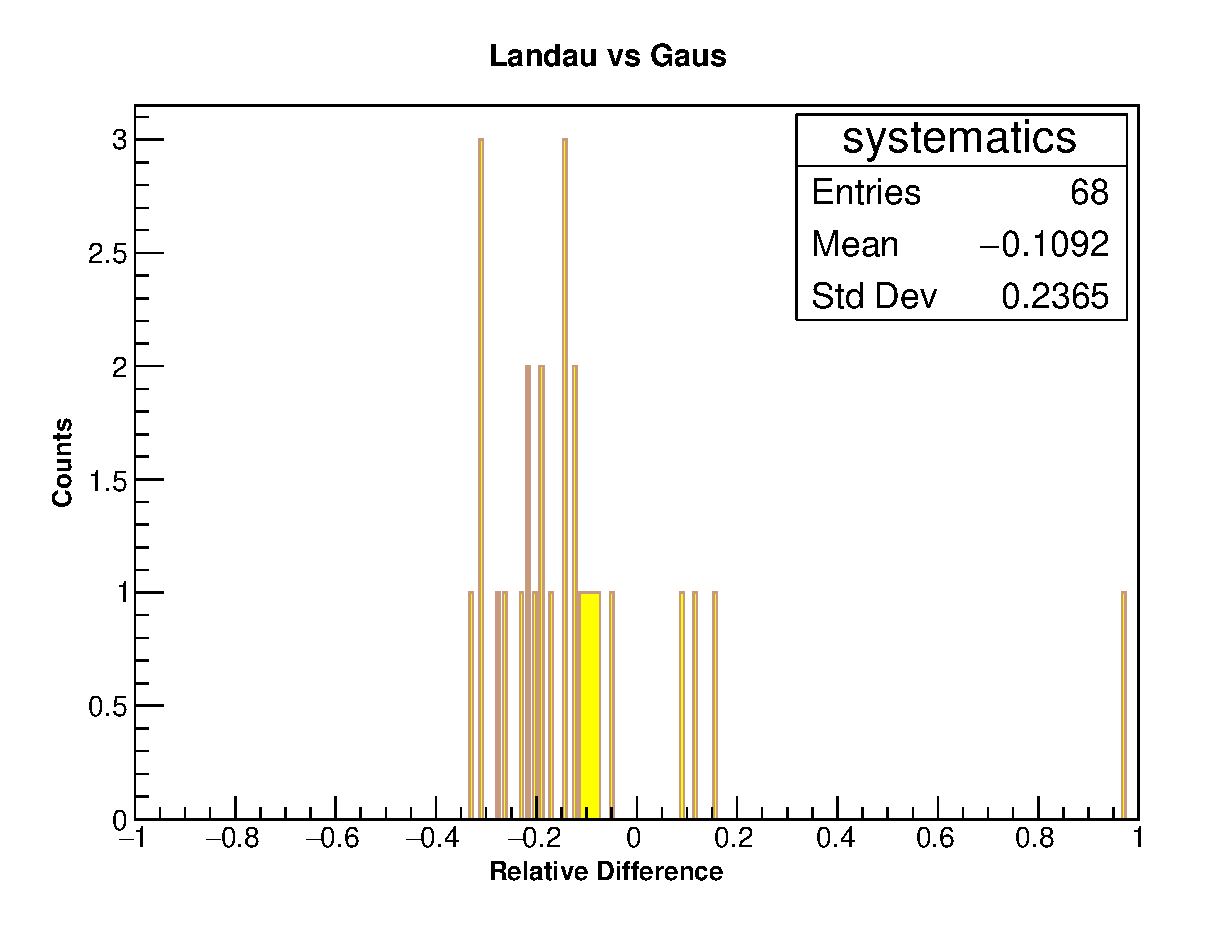
\includegraphics[width=\textwidth, height = 2.5in, keepaspectratio = true]{lanVgaus}
    \caption{Shown in the systematic effect in the differential cross section when
    using a Landau function over all passes relative to when using a Gaussian function.}
    \label{fig:lanVgaus}
    % plot created using /home/chetry/EC_PCAL/PCALanalysis_inC_taya/com/sys.c
\end{figure}

Words Words Words Words Words Words Words Words Words Words Words Words Words Words Words
Words Words Words Words Words Words Words Words Words Words Words Words Words Words Words 
Words Words Words Words Words Words Words Words Words Words Words Words Words Words Words 
Words Words Words Words Words Words Words Words Words Words Words Words Words Words Words.